67. а) Это прямоугольник, ограниченный прямыми $x=3,\ x=9,\ y=-3,\ y=6.$
$$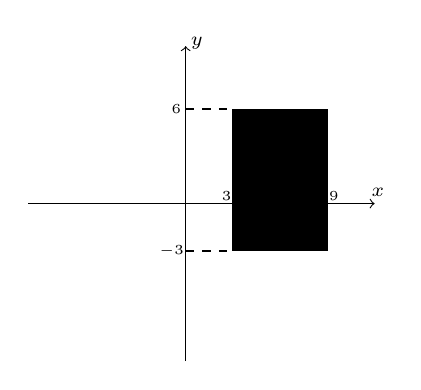
\begin{tikzpicture}[scale=0.2]
\tikzset {line01/.style={line width =0.5pt}}
\tikzset{line02/.style={line width =1pt}}
\tikzset{line03/.style={dashed,line width =0.5pt}}
%\filldraw [black] (0,0) circle (1pt);
\draw [->] (-10,0) -- (12,0);
\draw [->] (0,-10) -- (0,10);
\filldraw [draw=black] (3,-3) rectangle (9,6);
\draw[line03] (0,-3) -- (3,-3);
\draw[line03] (0,6) -- (3,6);
%\draw[line03] (-1,0) -- (-1,1);
%\draw[line01] (0,-3) -- (-2,5);
%\draw (0.6,-4) node {\tiny $-4$};
%\draw (-1.6,-0.7) node {\tiny $-1$};
\draw (12.2,0.7) node {\scriptsize $x$};
\draw (2.6,0.5) node {\tiny $3$};
\draw (-0.9,-3) node {\tiny $-3$};
\draw (-0.6,6) node {\tiny $6$};
\draw (9.4,0.5) node {\tiny $9$};
%\draw (-2.2,1) node {\tiny $-\frac{3}{2}$};
\draw (0.7,10.2) node {\scriptsize $y$};
\end{tikzpicture}$$
б) Горизонтальная сторона этого прямоугольника равна $a+6-a=6,$ а вертикальная --- $2a-(-a)=3a.$ Он является квадратом при $3a=6,\ a=2.$\\
